\begin{figure}[!ht]
    \centering
    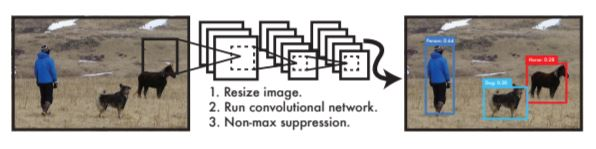
\includegraphics[width=0.7\textwidth]{chapter2/images/yolo.jpg}
    \caption{กระบวนการทำงานของโครงสร้างโมเดลปัญญาประดิษฐ์ของ YOLO}
    \label{fig:yolo}
\end{figure}

โครงสร้างโมเดลปัญญาประดิษฐ์ของ YOLO\textsuperscript{\cite{yolov3}} เป็นโครงสร้างที่มีความเร็วในการประมวลผลถึง 45 เฟรมต่อวินาที ทำให้สามารถประมวลผลแบบเรียลไทม์ได้ นอกจากนั้นยังมีความแม่นยำ mAP 
มากกว่าโมเดลสำหรับตรวจจับวัตถุอื่นๆถึง 2 เท่า ซึ่งเหตุผลที่โครงสร้างโมเดลปัญญาประดิษฐ์ของ YOLO เร็วกว่าโมเดลปัญญาประดิษฐ์ตัวอื่นๆ เนื่องจาก
การตรวจจับวัตถุในวิธีการก่อนหน้าจะใช้วิธีทำนายกรอบสี่เหลี่ยมก่อน แล้วจึงค่อยนำกรอบสี่เหลี่ยมไปทำนายว่าเป็นหมวดหมู่อะไร ซึ่ง YOLO มีวิธีการที่ต่างออกไป คือ 
ทำนายตำแหน่งของกรอบสี่เหลี่ยมและทำนายว่าเป็นหมวดหมู่อะไรพร้อมกัน โดยใช้โครงข่ายประสาทแบบคอนโวลูชัน ด้วยแนวคิดนี้จึงเป็นที่มาของชื่อ YOLO 
หรือ you only look once
\subsubsection*{โครงสร้างของโมเดลปัญญาประดิษฐ์ของ YOLO} 
\begin{figure}[!ht]
    \centering
    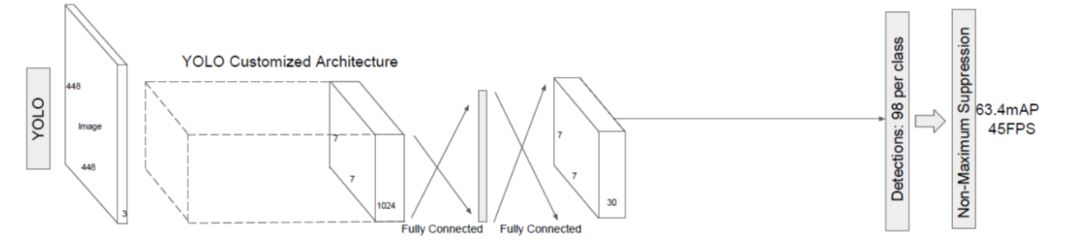
\includegraphics[width=0.7\textwidth]{chapter2/images/yolo_architecture.jpg}
    \caption{โครงสร้างทั่วไปของโมเดลปัญญาประดิษฐ์ของ YOLO}
    \label{fig:yolo_architecture}
\end{figure}

จากรูปภาพที่ \ref{fig:yolo_architecture} จะเห็นได้ว่า YOLO ใช้โครงข่ายประสาทเทียมเพียงตัวเดียวซึ่งภายในโครงข่ายจะมีกระบวนการหลักๆอยู่สามอย่าง 
กระบวนการแรกคือการสกัดคุณลักษณะ กระบวนการนี้จะมีจำนวนชั้นของเลเยอร์ที่แตกต่างกันไปตามความลึกของการสกัดแล้วแต่โมเดล ซึ่งตัวอย่างจะเป็นดังรูปที่ \ref{fig:yolo-architecture} 
และขั้นตอนถัดมาคือการทำนายผล หลังจากที่ได้คุณลักษณะมาแล้วจะนำไปทำนายผลผ่านชั้น fully connected ซึ่งจะได้ผลลัพธ์เป็นหมวดหมู่และตำแหน่งของกรอบสี่เหลี่ยม 
และขั้นตอนสุดท้ายคือการทำ NMS เพื่อให้ได้ผลลัพธ์ที่ดีที่สุดออกมา
\clearpage
\par ซึ่งโครงสร้างโมเดลปัญญาประดิษฐ์ของ YOLO ที่ถูกใช้ในงานวิจัยนี้ประกอบไปด้วย YOLO-v3 tiny, YOLO-v3 และ YOLO-v3 spp ซึ่งทั้งสามโครงสร้างจะแตกต่างดังนี้
\begin{enumerate}
	\setlength\itemsep{-0.25em}
	\item YOLO-v3 tiny ใช้ชั้น max pooling ในขั้นตอนของการลดจำนวนข้อมูลตัวอย่าง
	\item YOLO-v3 ใช้ชั้นคอนโวลูชั่น ในขั้นตอนของการลดจำนวนข้อมูลตัวอย่าง
	\item YOLO-v3 spp ใช้ชั้นคอนโวลูชั่น และคุณลักษณะที่ดีที่สุดของ max pooling ในขั้นตอนของการลดจำนวนข้อมูลตัวอย่าง
\end{enumerate}

\begin{figure}[!ht]
    \centering
    \begin{subfigure}[b]{0.2\textwidth}
        \centering
        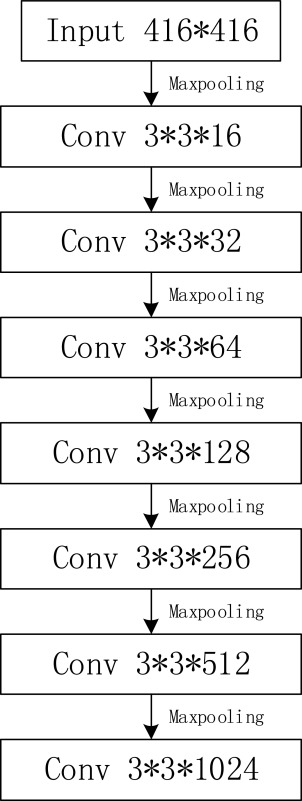
\includegraphics[width=\textwidth]{chapter2/images/yolo_tiny.jpg}
	 \caption{โครงสร้างโมเดลปัญญาประดิษฐ์ของ YOLO-v3 tiny}
        \label{fig:tiny}
    \end{subfigure}
    \begin{subfigure}[b]{0.3\textwidth}
        \centering
        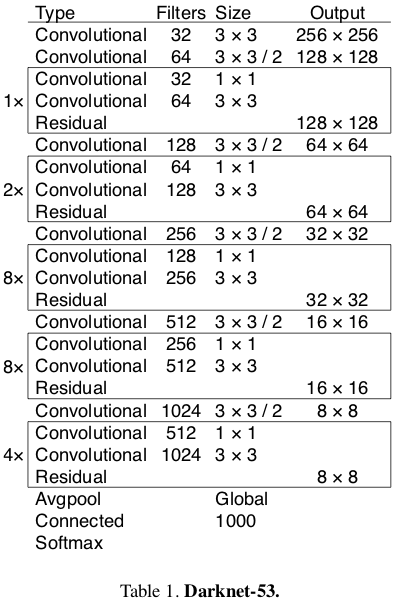
\includegraphics[width=\textwidth]{chapter2/images/yolo_darknet.png}
	 \caption{โครงสร้างโมเดลปัญญาประดิษฐ์ของ YOLO-v3}
       \label{fig:darknet}
    \end{subfigure}
    \begin{subfigure}[b]{0.5\textwidth}
        \centering
        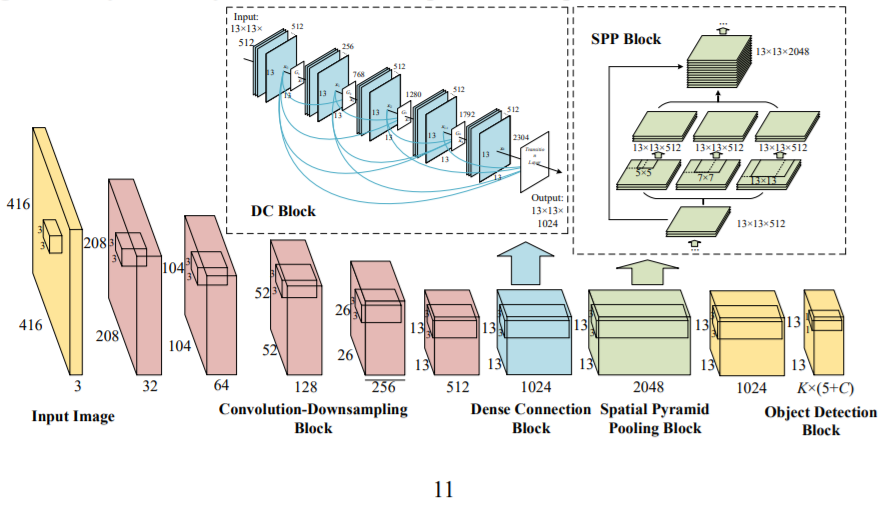
\includegraphics[width=\textwidth]{chapter2/images/yolo_spp.png}
	 \caption{โครงสร้างโมเดลปัญญาประดิษฐ์ของ YOLO-v3 spp}
       \label{fig:spp}
    \end{subfigure}
    \caption{โครงสร้างโมเดลปัญญาประดิษฐ์ของ YOLO}
    \label{fig:yolo-architecture}
\end{figure}

